\chapter{Experiments} \label{chapter:experiments}

The following section describes the setups of the experiments conducted with the neural network presented in chapter \ref{chapter:semi_automatic}. Due to the lack of existing annotated medical data the focus of the experiments is to ascertain a network design and mode of operation that compensate this as best as possible. First, we test the different network architectures that were described in section \ref{section:network_variations} using the same parameters. We then choose the best architecture for further experiments, in which we evaluate the two different training schemes introduced in section \ref{section:modes_of_operation}: training from scratch and incremental training.

\section{Terminology}

\noindent\textbf{Hyper Parameter.} \textit{Hyper parameters} are the tunable parameters of a network. The number and kind of parameters varies with the used type of network architecture, optimizer, etc.

\section{Datasets}


\begin{figure}[!tbp]
	\centering
	\begin{subfigure}[t]{0.47\textwidth}
		\centering
    	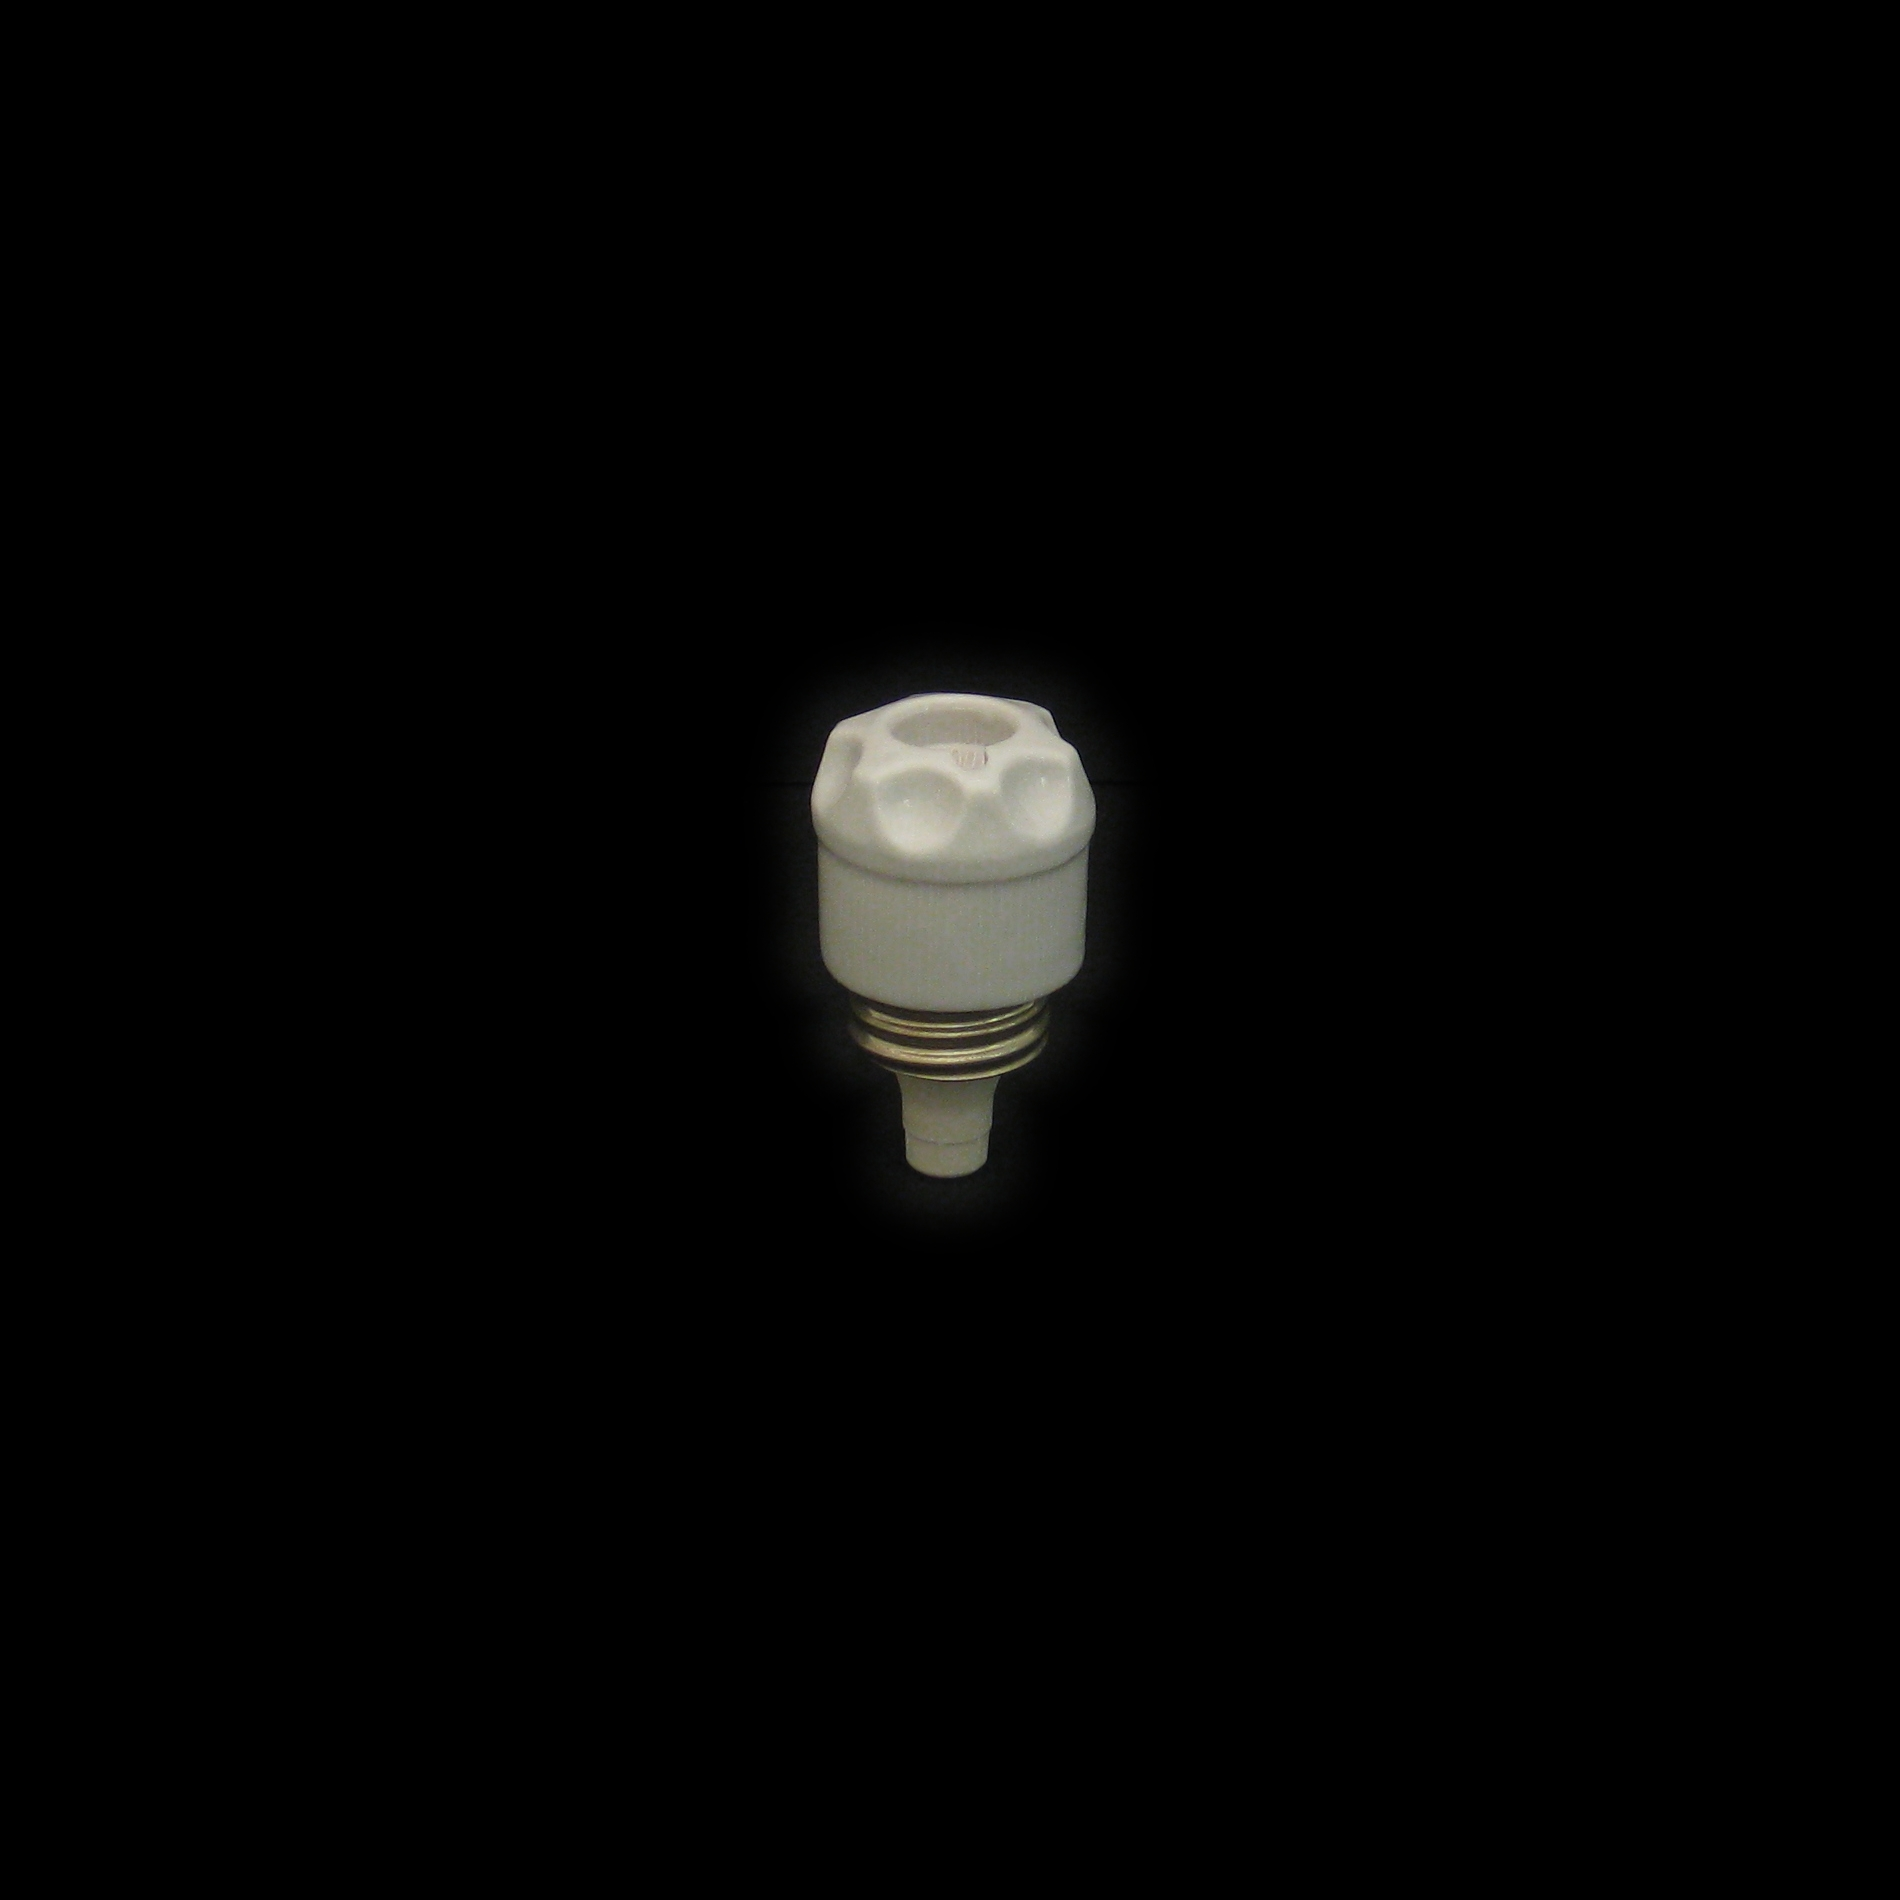
\includegraphics[width=0.6\linewidth]{tless_example_train}
    	\caption{An example frame from the training dataset of T-Less.}
    	\label{fig:tless_example_train}
	\end{subfigure}
	\hfill
	\begin{subfigure}[t]{0.47\textwidth}
		\centering
    	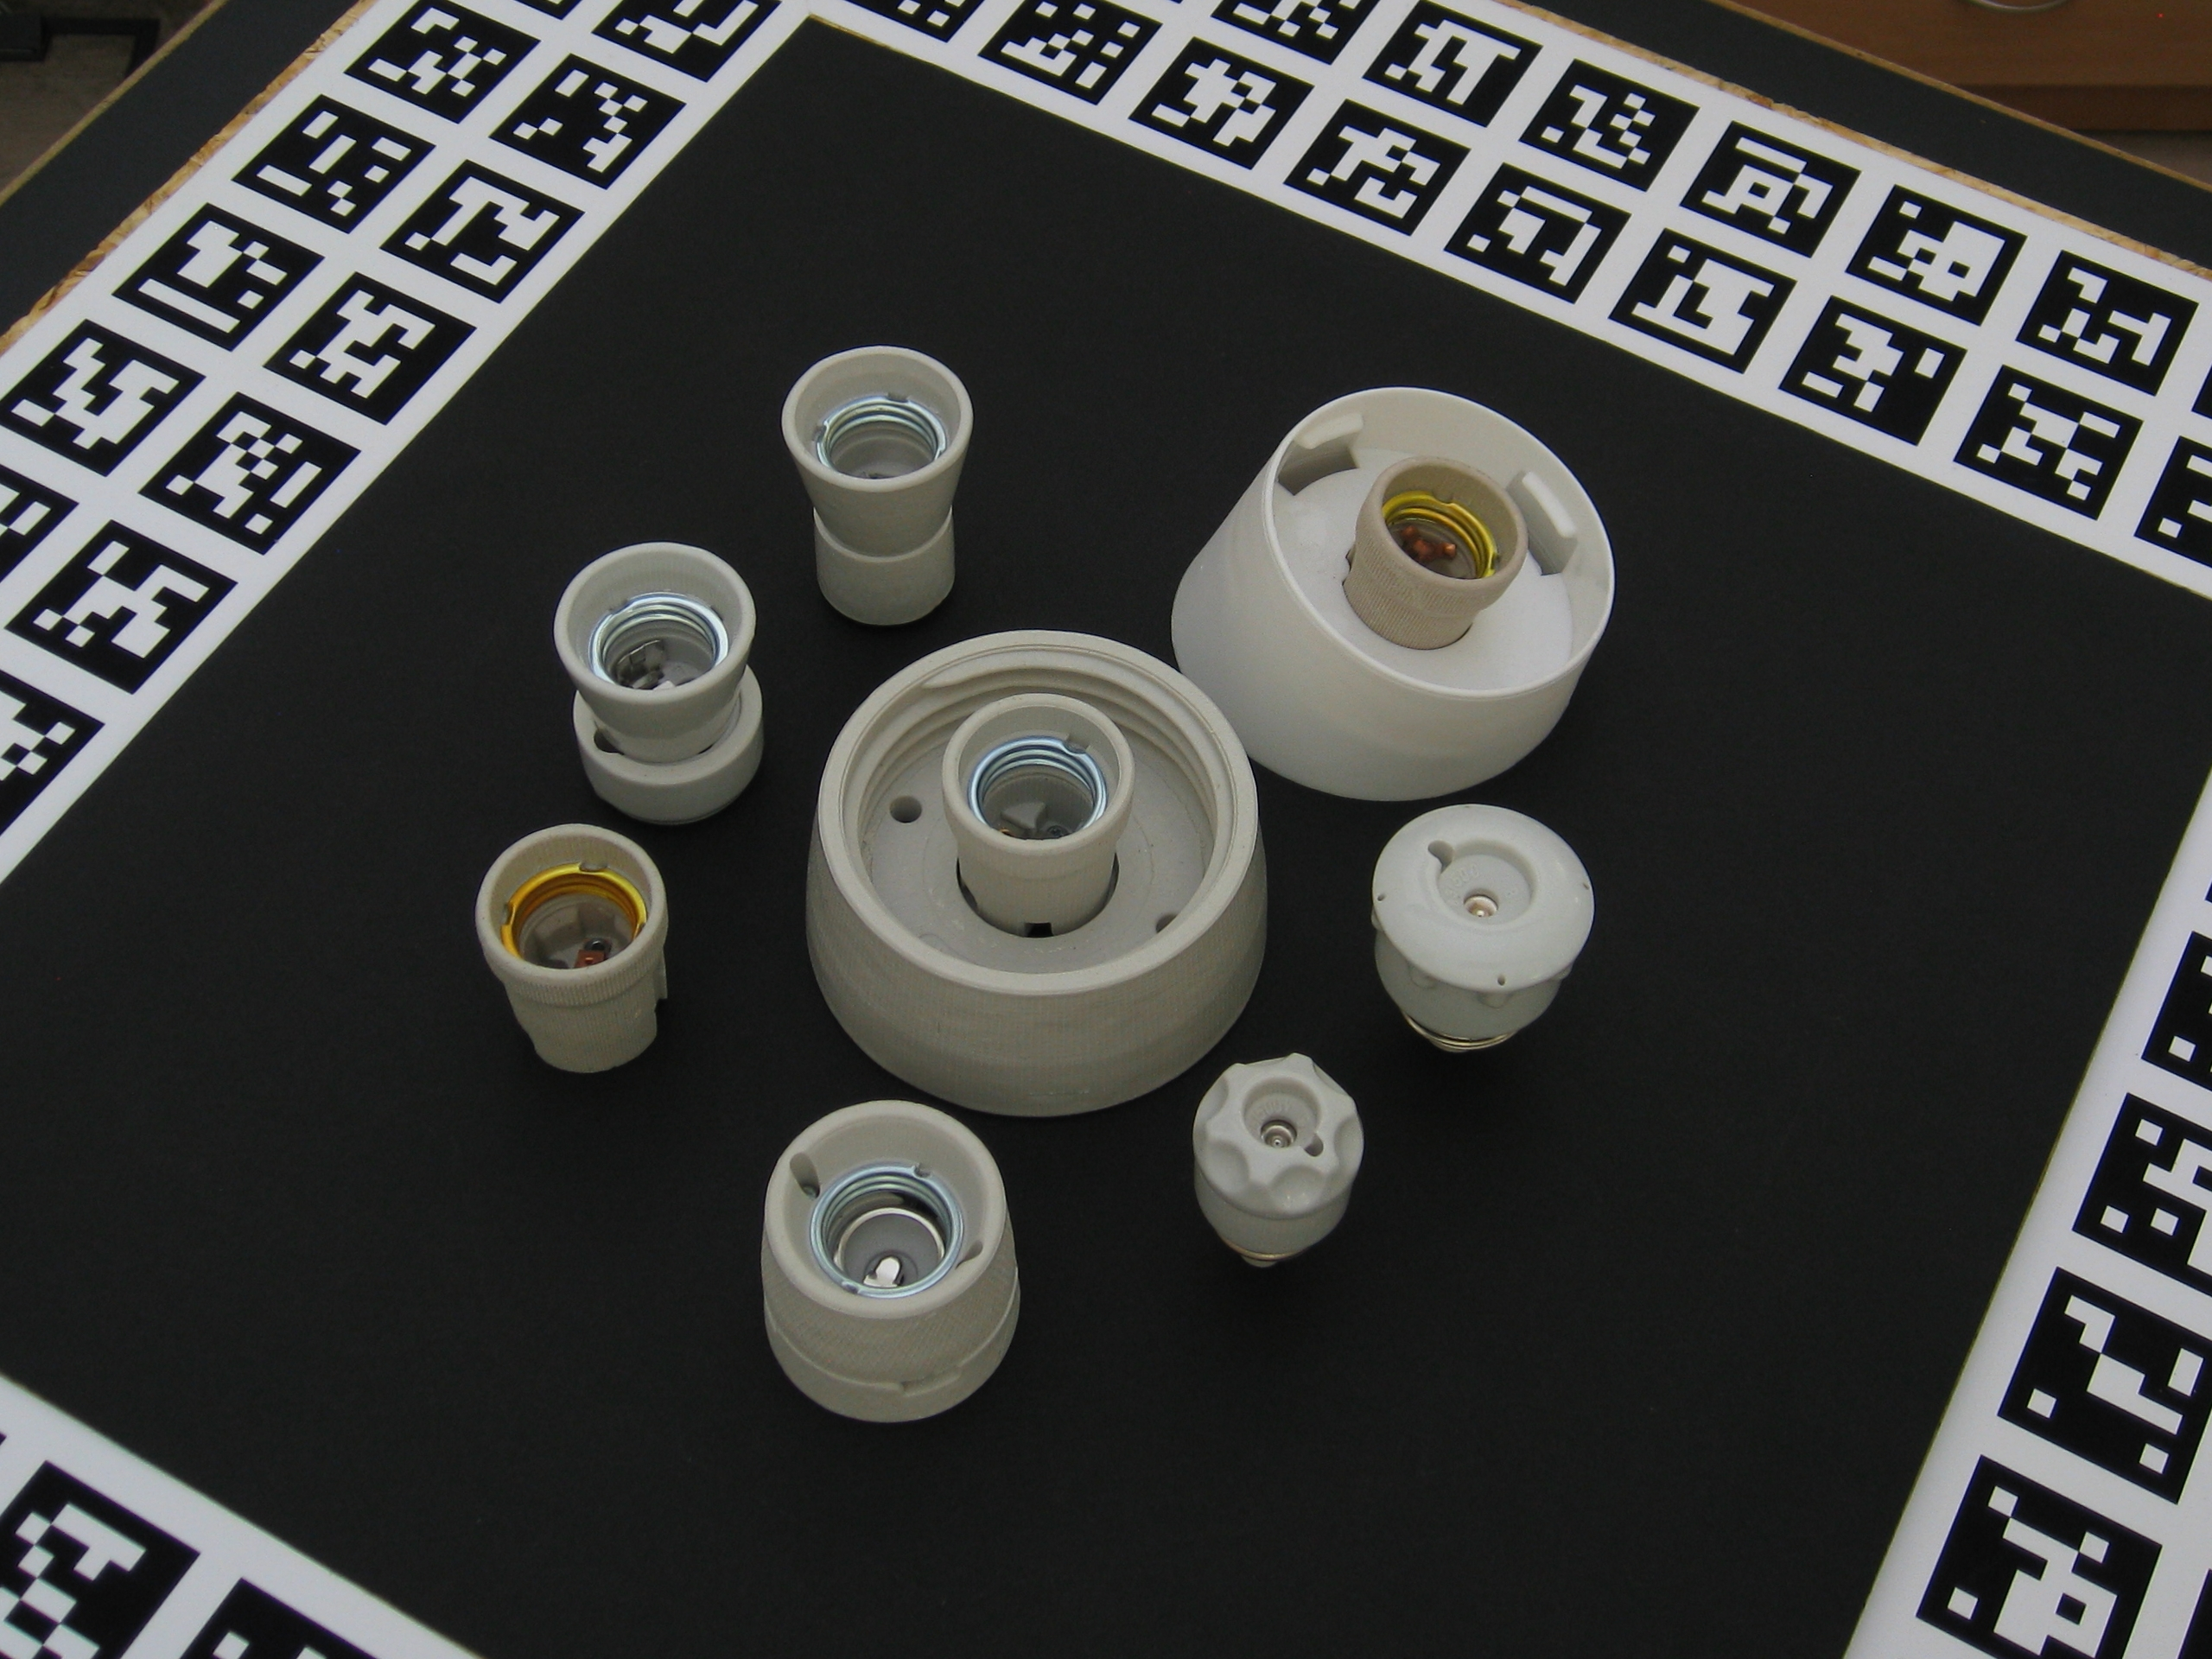
\includegraphics[width=0.7\linewidth]{tless_example_test}
    	\caption{An example frame from the test dataset of T-Less.}
    	\label{fig:tless_example_test}
	\end{subfigure}
	\caption{Example frames from the T-Less dataset \cite{tless}.}
	\label{fig:tless_examples}
\end{figure}

The initial intention to completely annotate the medical images provided at the beginning of the project turned out to be not feasible (see chapter \ref{chapter:manual_annotation}). Instead, we chose the T-Less dataset to conduct the experiments with. Its objects are mostly texture-less  and of rather small size making them similar to surgical tools. Next to many human pose estimation datasets, there exist some datasets of objects too, like \cite{next_view_dataset}, \cite{pracsys_dataset} and \cite{rigid_body_dataset}. But those resemble surgical tools less than the objects of the T-Less dataset.

The T-Less dataset was released in 2017 by Hoda\v{n} et al. \cite{tless}. It contains the object models of 30 industry-relevant real world objects. Two versions exist: one mesh of the object that was manually reconstructed using CAD software and one that was produced from RGB-D images. The objects were captured using a Primsense CARMINE 1.09, a Microsoft Kinect v2 and a Canon IXUS 950 IS. We used the photos of the Canon camera due to their quality and we do not need depth information, which is also provided by the CARMINE sensor and the Kinect. There are 1296 images of each object in the training set of the dataset, sampled in 10 degree steps in elevation and 5 degree azimuth. 20 test scenes, consisting of 504 images each, exist as well. Those are photographs of cluttered scenes of different complexity, with sometimes more than 15 objects visible. All training and test images are annotated with the ground-truth poses of the visible objects. The authors also provided a tool set to render the objects at a given pose, etc. Fig. \ref{fig:tless_example_train} shows an example frame from the training set and fig. \ref{fig:tless_example_test} an example frame from the test set. The training images of the other objects look similar to the one shown. The dataset provides depth images, as well, but this is irrelevant to our setting.

\section{Data Preparation}

The \textit{T-Less} dataset does not provide 3D object coordinates. This is the reason why we rendered them ourselves. The script is part of the network package. Segmentation masks were rendered as well. Because the 32-bit TIFF object coordinate ground-truth files used up too much disk space when in original size they were cropped to the relevant area by determining the smallest box around the segmentation pixels. Because a part of the dataset had to be cropped the author of this worked deemed it best to crop all input to the respective segmentation masks. As a result, the network expects all input to be cropped. Or, to be precise, the size that the network is configured to expect as input has to be larger than the size of the segmentation images. The network runs with other configurations but doesn't produce any usable output in this case. There are no other alterations made to the data.

\section{Training Experiments}

This section describes the configuration of the different training experiments, i.e. which model was used, how many images, etc. The chronological order of the experiments is reflected here. First, we compare the \gls{sgd} and Adam optimizer in \ref{subsection:optimizers}. Then we evaluate the different architectures against each other in \ref{subsection:architectures}. Finally, asses the two training strategies training from scratch and incremental training in \ref{subsection:training_strategies}.

\subsection{Optimizers} \label{subsection:optimizers}

We used the first network architecture to compare the \gls{sgd} and Adam optimizer. The first network architecture consists of 23 layers and has a receptive field-size of 99 per output pixel. The decreasing learning rates for \gls{sgd} were set to ... TODO: insert learning rates, $\beta_1$ and $\beta_2$ of the Adam optimizer were left at the default values set by Keras, which are $0.9$ and $0.999$, respectively. Fig. \ref{todo} shows the loss of both experiments during training. Since Adam declines much faster than \gls{sgd}, we chose Adam as the optimizer for all other experiments.

\subsection{Loss Functions}

% L1 vs L2 loss

\subsection{Architectures} \label{subsection:architectures}

The experiments run on the different architectures were all performed using the Adam optimizer with the parameters mentioned above. The major difference between the experiments is the architecture itself. The training process were run for a different number of iterations because some architectures converged earlier than others. The different losses are displayed in fig. \ref{todo}.

\subsection{Training Strategies} \label{subsection:training_strategies}

% Nochmal zusammenfassen scratch vs inkrementell

\subsection{Limitations}

% No challenge yet, difficult to tell how good network is -> no baseline!

% T-Less dataset contains only unoccluded images

% This way of comparing is owned to the timeframe of this work -> maybe L2 works better for model 5, etc. 

% Create metric for images that the network produces bad predictions for, e.g. reprojection error for contradicting object coordinates, difference between segmentation mask rendered using the predicted pose and the ground-truth segmentation mask -> was not possible because we couldn't annotate images of the Endovis dataset

\subsection{Runtime Analysis}

This section analyses the inference runtimes of the different architectures. Deeper networks need longer to perform training and an inference run on an image, which is reflected by table ...